\section{\trAdjunction}
\label{sec:adjunctions}

在本节中，我们将讨论∞-\trCategories{}之间的\trAdjunction{}。我们将以%
\trFibration{}的语言来定义它们，并证明它们也可以等价地描述为：对%
\trBivariant{}\trMappingSpace{}\trFunctor{}选取一个%
\trBinaturalTransformation{}（binatural transformation）。
对于给定的\trFunctor{} $f\colon \C \to \D$，我们将仿照通常\trCategoryTheory{}%
中的做法，给出若干使 $f$ 容许伴随的充分判据，并讨论一些例子。此外，我们将证明
（余）\trLimit{}（如果存在的话）可以被\trFunctor{}式地构造出来：为此只需证明
它们的构造装配成\trDiagonalFunctor{}（diagonal functor）或%
\trConstantFunctor{}的一个伴随。最后，我们将讨论\trBousfield{}\trLocalization{}%
的概念，即那些容许\trRightAdjoint{}的\trDwyer{}--\trKan{}\trLocalization{}，
或者等价地，那些容许\trFullyFaithful{}\trRightAdjoint{}的\trFunctor{}。

\begin{definition}\label{def:adjunction-infinity}
一个\emph{\trAdjunction{}}（adjunction）是一个\trBicartesianFibration{}%
（bicartesian fibration）$\E \to \Delta^1$，也就是说，是一个既是%
\trCartesianFibration{}又是\trCocartesianFibration{}的\trFunctor{}。
\end{definition}

\begin{definition}\label{def:left-right-adjoint}
给定一个\trAdjunction{}，我们可以利用\trStraightening{}--\trUnstraightening{}%
\trEquivalence{}得到一个由该\trCocartesianFibration{}所分类的\trFunctor{}%
$f\colon \E_0 \to \E_1$，同样也可以得到一个由该\trAdjunction{}的底层%
\trCartesianFibration{}所分类的\trFunctor{} $g\colon \E_1 \to \E_0$。我们称
$f$ 为该\trAdjunction{}的\trLeftAdjoint{}，称 $g$ 为其\trRightAdjoint{}。
\end{definition}

\begin{remark}\label{rem:admits-right-adjoint}
我们说一个\trFunctor{} $f\colon \C \to \D$ 容许一个\trRightAdjoint{}，如果存在
一个\trAdjunction{} $\E \to \Delta^1$，其相伴\trFunctor{}等价于 $f$；也就是说，
在其中指定了\trEquivalence{} $\C \simeq \E_0$ 与 $\D \simeq \E_1$，使得复合
$\C \simeq \E_0 \to \E_1 \simeq \D$ 等价于 $f$。于是一般地，两个∞-\trCategories{}%
$\C$ 与 $\D$ 之间的一个\trAdjunction{}由一个\trBicartesianFibration{}%
$\E \to \Delta^1$
连同指定的\trEquivalence{} $\C \simeq \E_0$ 与 $\D \simeq \E_1$ 一道构成。
\end{remark}

\begin{remark}\label{rem:adjunction-map-equivalence}
我们可以直接证明：一个\trAdjunction{} $\E \to \Delta^1$ 给出诸空间的一个%
\trEquivalence{}%
\[
\mathrm{map}_{\E_1}(f(x), z) \simeq \mathrm{map}_{\E_0}(x, g(z)),
\]
其中 $x$ 是 $\E_0$ 的一个\trObject{}，而 $z$ 是 $\E_1$ 的一个\trObject{}。为此，
我们考虑诸空间 $\mathrm{map}_{\E}(x, z)$。选取唯一映射 $0 \to 1$ 的一个以 $z$
为靶的笛卡尔提升，由第 3 章中的\cref{cor:cartesian-lift-mapping-fibre}我们发现
存在一个\trFibreSequence{}%
\[
\mathrm{map}_{\E_0}(x, g(z)) \longrightarrow \mathrm{map}_{\E}(x, z)
  \longrightarrow \mathrm{map}_{\Delta^1}(0, 1) \simeq *,
\]
于是其中第一个映射是一个\trHomotopyEquivalence{}。同样地，选取一个以 $x$ 为源的
余笛卡尔提升，便给出一个\trFibreSequence{}%
\[
\mathrm{map}_{\E_1}(f(x), z) \longrightarrow \mathrm{map}_{\E}(x, z)
  \longrightarrow \mathrm{map}_{\Delta^1}(0, 1) \simeq *.
\]
于是，我们以下述之字形（zig-zag）得到所要的\trEquivalence{}%
\[
\mathrm{map}_{\E_1}(f(x), z) \xrightarrow{\ \simeq\ } \mathrm{map}_{\E}(x, z)
  \xleftarrow{\ \simeq\ } \mathrm{map}_{\E_0}(x, g(z)).
\]
\end{remark}

现在，我们想把这个结果提升为诸\trFunctor{}%
$\E_0^{\mathrm{op}} \times \E_1 \to \mathrm{Spc}$ 的一个\trNaturalEquivalence{}。

\begin{proposition}\label{prop:adjunction-map-natural-equivalence}
设 $\E \to \Delta^1$ 是一个\trAdjunction{}，其相伴\trFunctor{}为
$f\colon \E_0 \to \E_1$ 与 $g\colon \E_1 \to \E_0$。那么，存在诸\trFunctor{}的
一个\trNaturalEquivalence{}%
\[
\mathrm{map}_{\E_0}(-, g(-)) \simeq \mathrm{map}_{\E_1}(f(-), -).
\]
\end{proposition}

\begin{proof}
我们断言，这两个\trFunctor{}都等价于复合
\[
\E_0^{\mathrm{op}} \times \E_1 \longrightarrow \E^{\mathrm{op}} \times \E
  \longrightarrow \mathrm{Spc},
\]
其中后者是∞-\trCategory{} $\E$ 的\trBivariant{}\trMappingSpace{}\trFunctor{}。
为此，我们
首先注意到，存在诸\trFunctor{}的\trNaturalTransformation{}%
$\tau_g\colon i_0 \circ g \to i_1$ 与 $\tau_f\colon i_0 \to i_1 \circ f$，它们
挑出所需要的（余）笛卡尔映射：考虑图表
\begin{center}
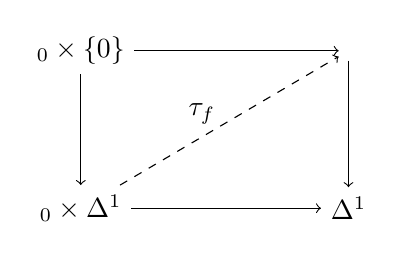
\begin{tikzpicture}
  \node (tl) at (0,0) {$\E_0 \times \{0\}$};
  \node (tr) at (3.4,0) {$\E$};
  \node (bl) at (0,-2.0) {$\E_0 \times \Delta^1$};
  \node (br) at (3.4,-2.0) {$\Delta^1$};
  \draw[->] (tl) -- (tr);
  \draw[->] (tl) -- (bl);
  \draw[->] (bl) -- (br);
  \draw[->] (tr) -- (br);
  \draw[->, dashed] (bl) -- node[pos=0.45, above left, inner sep=1pt]
    {$\tau_f$} (tr);
\end{tikzpicture}
\qquad
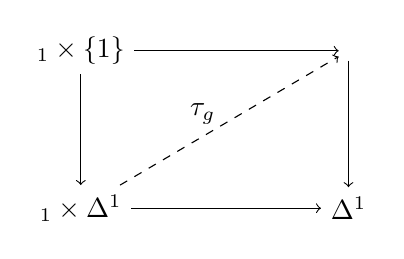
\begin{tikzpicture}
  \node (tl) at (0,0) {$\E_1 \times \{1\}$};
  \node (tr) at (3.4,0) {$\E$};
  \node (bl) at (0,-2.0) {$\E_1 \times \Delta^1$};
  \node (br) at (3.4,-2.0) {$\Delta^1$};
  \draw[->] (tl) -- (tr);
  \draw[->] (tl) -- (bl);
  \draw[->] (bl) -- (br);
  \draw[->] (tr) -- (br);
  \draw[->, dashed] (bl) -- node[pos=0.45, above left, inner sep=1pt]
    {$\tau_g$} (tr);
\end{tikzpicture}
\end{center}
其中虚箭头之所以存在，是因为 $\E^{\E_i} \to \Delta^{\E_i}$ 仍是双笛卡尔的，于是
我们便找到所要的这类提升。随后，我们考虑复合
\[
\E_0^{\mathrm{op}} \times \E_1 \times \Delta^1
  \to \E_0^{\mathrm{op}} \times \E
  \to \E^{\mathrm{op}} \times \E \to \mathrm{Spc},
\]
它是从 $\mathrm{map}_{\E}(-, g(-))$ 到 $\mathrm{map}_{\E}(-, -)$ 的一个%
\trNaturalTransformation{}。由于 $\tau_g$ 是逐点的笛卡尔边，它是一个逐点%
\trEquivalence{}。利用「$i_0\colon \E_0 \to \E$ 是\trFullyFaithful{}（%
$\Delta^1$ 的诸自映射空间是平凡的）」以及「逐点为等价的%
\trNaturalTransformation{}本身是等价（见第 2 章中的%
\cref{cor:pointwise-equivalences}）」，我们得出结论：$\tau_g$ 诱导一个%
\trNaturalEquivalence{}%
\[
\mathrm{map}_{\E_0}(-, g(-)) \simeq \mathrm{map}_{\E}(-, -)\colon
  \E_0^{\mathrm{op}} \times \E_1 \to \mathrm{Spc}.
\]
同样地，$\tau_f$ 诱导一个\trNaturalEquivalence{}%
\[
\mathrm{map}_{\E_1}(f(-), -) \simeq \mathrm{map}_{\E}(-, -)\colon
  \E_0^{\mathrm{op}} \times \E_1 \to \mathrm{Spc},
\]
断言即证。
\end{proof}

接下来，我们想定义与一个\trAdjunction{}相伴的\trUnit{}变换与\trCounit{}变换。
如同\cref{prop:adjunction-map-natural-equivalence}的证明中那样，我们考虑变换
$\tau_f$ 与 $\tau_g$，并且观察到：下述两个映射
\begin{center}
\begin{tikzpicture}
  \node (tl) at (0,0) {$\E_1 \times \Delta^1$};
  \node (tr) at (4.0,0) {$\E$};
  \node (bl) at (0,-2.1) {$\E_0 \times \Delta^1$};
  \draw[->] (tl) -- node[above] {$\tau_g$} (tr);
  \draw[->] (tl) -- node[left] {$g \times \mathrm{id}$} (bl);
  \draw[->] (bl) -- node[below right, inner sep=1pt] {$\tau_f$} (tr);
\end{tikzpicture}
\end{center}
在限制到 $\E_1 \times \{0\}$ 上时是同一个映射：由定义，$\tau_g$ 限制为%
\trFunctor{} $i_0 \circ g$，而 $\tau_f \circ (g \times \mathrm{id})$ 限制为 $g$
与包含 $i_0$ 的复合。

于是，这两个映射拼合成一个映射 $\E_1 \times \Lambda_0^2 \to \E$，它限制在
$\E_1 \times \Delta^{(0,1)}$ 上由 $\tau_f \circ (g \times \mathrm{id})$ 给出，
而限制在 $\E_1 \times \Delta^{(0,2)}$ 上由 $\tau_g$ 给出。这就给出了下述图表中
上方的水平映射
\begin{center}
\begin{tikzpicture}
  \node (tl) at (0,0) {$\E_1 \times \Lambda_0^2$};
  \node (tr) at (4.4,0) {$\E$};
  \node (bl) at (0,-2.0) {$\E_1 \times \Delta^2$};
  \node (br) at (4.4,-2.0) {$\Delta^1$};
  \draw[->] (tl) -- (tr);
  \draw[->] (tl) -- (bl);
  \draw[->] (bl) -- (br);
  \draw[->] (tr) -- (br);
  \draw[->, dashed] (bl) -- (tr);
\end{tikzpicture}
\end{center}
而下方的水平映射由复合 $\E_1 \times \Delta^2 \to \Delta^2 \to \Delta^1$ 给出，
其中后一个映射把 $0$ 送到 $0$，把 $1$ 与 $2$ 都送到 $1$。为了看出该图表交换，
只需回忆 $p \circ \tau_f$ 与 $p \circ \tau_g$ 都是投射。这时我们发现，这个%
\trLiftingProblem{}可以求解，因为复合
\[
\E_1 \times \Delta^{(0,1)} \longrightarrow \E_1 \times \Lambda_0^2
  \longrightarrow \E
\]
是逐点余笛卡尔的。对 $\E_1$ 的一个\trObject{} $z$，所得出的 $\E$ 的
$2$-\trSimplex{}由
\begin{center}
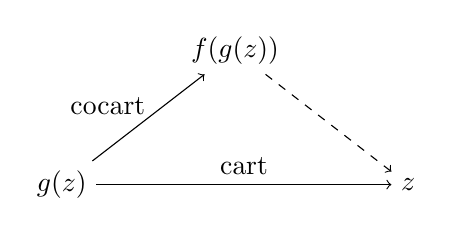
\begin{tikzpicture}
  \node (top) at (2.2,0) {$f(g(z))$};
  \node (bl) at (0,-1.7) {$g(z)$};
  \node (br) at (4.4,-1.7) {$z$};
  \draw[->] (bl) -- node[above left, inner sep=1pt] {cocart} (top);
  \draw[->, dashed] (top) -- (br);
  \draw[->] (bl) -- node[above] {cart} (br);
\end{tikzpicture}
\end{center}
给出。最后，由构造，限制 $\E_1 \times \Delta^{(1,2)} \to \E_1 \times \Delta^2 \to \E$
穿过包含 $\E_1 \to \E$ 而分解。

一个类似的构造提供了一个\trFunctor{} $\E_0 \times \Delta^2 \to \E_0$，它可以
描绘如下：
\begin{center}
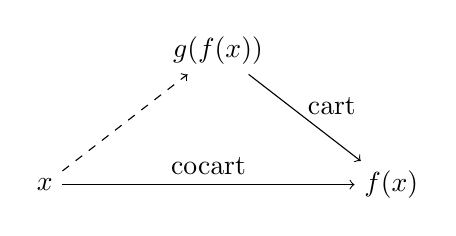
\begin{tikzpicture}
  \node (top) at (2.2,0) {$g(f(x))$};
  \node (bl) at (0,-1.7) {$x$};
  \node (br) at (4.4,-1.7) {$f(x)$};
  \draw[->, dashed] (bl) -- (top);
  \draw[->] (top) -- node[above right, inner sep=1pt] {cart} (br);
  \draw[->] (bl) -- node[above] {cocart} (br);
\end{tikzpicture}
\end{center}

\begin{definition}\label{def:unit-counit}
我们把所得的\trFunctor{} $\varepsilon\colon \E_1 \times \Delta^1 \to \E_1$ 称为
该\trAdjunction{}的\emph{\trCounit{}}（counit）。对偶地，我们把所得的%
\trFunctor{} $\eta\colon \E_0 \times \Delta^1 \to \E_0$ 称为该\trAdjunction{}%
的\emph{\trUnit{}}（unit）。
\end{definition}

\begin{remark}\label{rem:cartesian-lift-not-cocartesian}
在一个\trAdjunction{} $\E \to \Delta^1$ 中，唯一的\trMorphism{} $0 \to 1$ 既有
笛卡尔提升又有余笛卡尔提升。然而一般地，一个笛卡尔提升未必是余笛卡尔的，反之
亦然。事实上，这一点可以被很好地控制。
\end{remark}

\begin{proposition}\label{prop:cart-cocart-fully-faithful}
设 $p\colon \E \to \Delta^1$ 是一个\trAdjunction{}，其\trLeftAdjoint{}为
$f\colon \E_0 \to \E_1$，\trRightAdjoint{}为 $g\colon \E_1 \to \E_0$。那么，
$p$-笛卡尔边是 $p$-余笛卡尔的，当且仅当 $g$ 是\trFullyFaithful{}。反之，
$p$-余笛卡尔边是 $p$-笛卡尔的，当且仅当 $f$ 是\trFullyFaithful{}。特别地，
$f$ 与 $g$ 是互逆的\trEquivalence{}，当且仅当 $p$-笛卡尔边之集等于
$p$-余笛卡尔边之集。
\end{proposition}

\begin{proof}
我们先证明：笛卡尔边是余笛卡尔的，当且仅当\trCounit{}是一个\trEquivalence{}。
为此，考虑前文的那个 $2$-\trSimplex{}%
\begin{center}
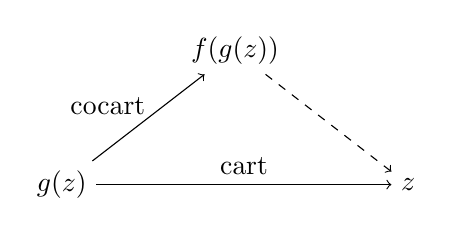
\begin{tikzpicture}
  \node (top) at (2.2,0) {$f(g(z))$};
  \node (bl) at (0,-1.7) {$g(z)$};
  \node (br) at (4.4,-1.7) {$z$};
  \draw[->] (bl) -- node[above left, inner sep=1pt] {cocart} (top);
  \draw[->, dashed] (top) -- (br);
  \draw[->] (bl) -- node[above] {cart} (br);
\end{tikzpicture}
\end{center}
并假设笛卡尔边都是余笛卡尔的。由第 3 章中的\cref{lem:cartesian-three-for-two}的对偶版本，
我们发现\trCounit{}映射 $f(g(z)) \to z$ 也是余笛卡尔的，从而对每个 $z$ 都是一个%
\trEquivalence{}，因为它的像在 $\Delta^1$ 中是\trInvertible{}。于是，%
\trCounit{}是一个%
\trNaturalEquivalence{}。反之，如果\trCounit{}是一个\trEquivalence{}，那么它也
是余笛卡尔的，于是笛卡尔边 $g(z) \to z$ 作为余笛卡尔边的复合也是余笛卡尔的。

接下来，我们将证明 $g$ 是\trFullyFaithful{}当且仅当\trCounit{}是一个%
\trEquivalence{}。由构造，图表
\begin{center}
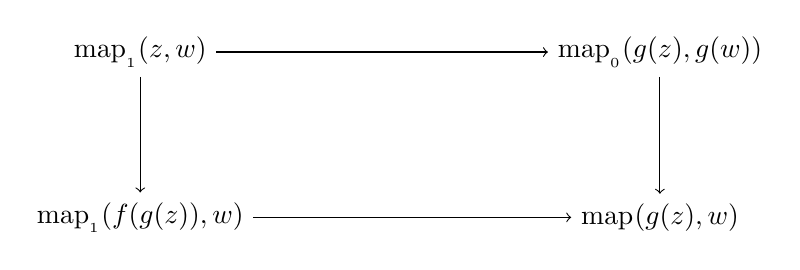
\begin{tikzpicture}
  \node (tl) at (0,0) {$\mathrm{map}_{\E_1}(z, w)$};
  \node (tr) at (6.6,0) {$\mathrm{map}_{\E_0}(g(z), g(w))$};
  \node (bl) at (0,-2.1) {$\mathrm{map}_{\E_1}(f(g(z)), w)$};
  \node (br) at (6.6,-2.1) {$\mathrm{map}_{\E}(g(z), w)$};
  \draw[->] (tl) -- (tr);
  \draw[->] (tl) -- (bl);
  \draw[->] (tr) -- (br);
  \draw[->] (bl) -- (br);
\end{tikzpicture}
\end{center}
交换。下方的水平映射与右边的竖直映射都是\trEquivalence{}，因为它们分别由与一条
笛卡尔边的后合成、或与一条余笛卡尔边的前合成所诱导。于是，$g$ 是%
\trFullyFaithful{}当且仅当\trCounit{}是一个\trEquivalence{}。

关于\trUnit{}的论证是类似的，而「特别地」部分则由下述事实得出：$f$ 与 $g$
互逆，当且仅当二者都是\trFullyFaithful{}。
\end{proof}

\begin{definition}\label{def:admit-adjoint-fibration}
设 $f\colon \C \to \D$ 是∞-\trCategories{}之间的一个\trFunctor{}。如果与 $f$
相伴的\trCocartesianFibration{} $\E \to \Delta^1$ 是笛卡尔的，我们就说 $f$
容许一个\trRightAdjoint{}。反之，如果与 $g$ 相伴的\trCartesianFibration{}%
$\E' \to \Delta^1$ 是余笛卡尔的，我们就说 $g\colon \D \to \C$ 容许一个%
\trLeftAdjoint{}。
\end{definition}

下面的命题提供了一个构造\trFunctor{}的有用办法。

\begin{proposition}\label{prop:right-adjoint-criterion}
设 $f\colon \C \to \D$ 是∞-\trCategories{}之间的一个\trFunctor{}。对 $\D$ 的
每个\trObject{} $x$，指定 $\C$ 的一个\trObject{} $gx$ 以及 $\D$ 中的映射
$f(gx) \to x$。如果诱导的复合
\[
\mathrm{map}_{\C}(z, gx) \xrightarrow{\ f\ } \mathrm{map}_{\D}(f(z), f(gx))
  \xrightarrow{\ \varepsilon\ } \mathrm{map}_{\D}(f(z), x)
\]
是一个\trEquivalence{}，那么存在一个\trFunctor{} $g\colon \D \to \C$，它把 $x$
送到 $gx$，并且是 $f$ 的\trRightAdjoint{}。此外，此时该\trAdjunction{}的%
\trCounit{}等价于
所选的映射 $f(gx) \to x$。
\end{proposition}

\begin{proof}
设 $p\colon \E \to \Delta^1$ 是与\trFunctor{} $f$ 相伴的%
\trCocartesianFibration{}。我们想证明 $p$ 是笛卡尔的。换句话说，对
$\E_1 \simeq \D$ 的每个\trObject{} $x$，我们必须在 $\Delta^1$ 的唯一非恒等%
\trMorphism{}之上指定一个 $p$-笛卡尔\trMorphism{}。为此，我们考虑
$\E_0 \simeq \C$ 的\trObject{} $gx$，并选取一条 $p$-余笛卡尔\trMorphism{}%
$gx \to f(gx)$。把这条\trMorphism{}与指定的\trMorphism{} $f(gx) \to x$ 复合，
我们便得到 $\Delta^1$ 的唯一非恒等\trMorphism{}之上的一个映射 $gx \to x$。如果
我们能证明这个映射是 $p$-笛卡尔的，那么本命题的第一部分即得。为此，注意：
$\E$ 中位于 $0 \to 1$ 之上的一条\trMorphism{} $\alpha\colon u \to v$ 是
$p$-笛卡尔的，当且仅当映射
\[
\mathrm{map}_{\E}(w, u) \xrightarrow{\ \alpha\ } \mathrm{map}_{\E}(w, v)
\]
对一切 $w \in \E_0$ 都是\trHomotopyEquivalence{}（例如利用第 3 章中的%
\cref{rem:cartesian-characterization}）。换句话说，我们必须证明：复合
\[
\mathrm{map}_{\E}(z, gx) \longrightarrow \mathrm{map}_{\E}(z, f(gx))
  \longrightarrow \mathrm{map}_{\E}(z, x)
\]
对一切 $z \in \E_0$ 都是一个\trEquivalence{}。为此，我们选取一条 $p$-余笛卡尔边
$z \to f(z)$，并考虑图表
\begin{center}
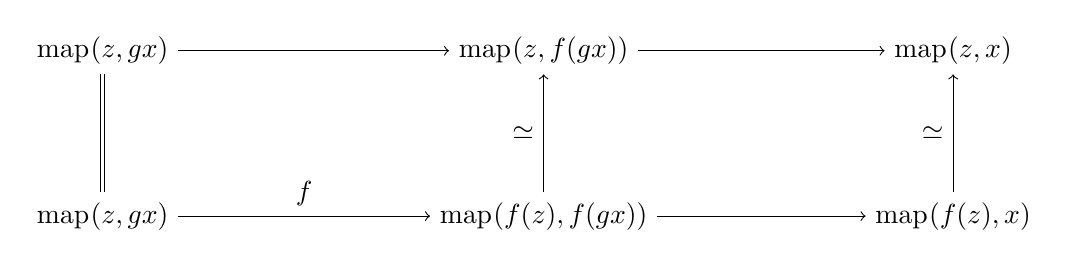
\begin{tikzpicture}
  \node (a) at (0,0) {$\mathrm{map}_{\E}(z, gx)$};
  \node (b) at (5.6,0) {$\mathrm{map}_{\E}(z, f(gx))$};
  \node (c) at (10.8,0) {$\mathrm{map}_{\E}(z, x)$};
  \node (d) at (0,-2.1) {$\mathrm{map}_{\E}(z, gx)$};
  \node (e) at (5.6,-2.1) {$\mathrm{map}_{\E}(f(z), f(gx))$};
  \node (f) at (10.8,-2.1) {$\mathrm{map}_{\E}(f(z), x)$};
  \draw[double, double distance=1.2pt] (a) -- (d);
  \draw[->] (d) -- node[above] {$f$} (e);
  \draw[->] (e) -- (f);
  \draw[->] (a) -- (b);
  \draw[->] (b) -- (c);
  \draw[->] (e) -- node[left] {$\simeq$} (b);
  \draw[->] (f) -- node[left] {$\simeq$} (c);
\end{tikzpicture}
\end{center}
其中中间的竖直映射与右边的竖直映射都是\trEquivalence{}，因为 $z \to f(z)$ 是
$p$-余笛卡尔的，而 $x$ 与 $f(gx)$ 是 $\E_1$ 的\trObject{}。下方的复合由假设是
一个\trEquivalence{}，故上方的复合也是一个\trEquivalence{}。于是，上面构造的
映射 $gx \to x$ 是 $p$-笛卡尔的。

剩下还需证明关于该\trAdjunction{}之\trCounit{}的断言。但这由构造即得：注意，
$\E$ 中有一个 $2$-\trSimplex{}%
\begin{center}
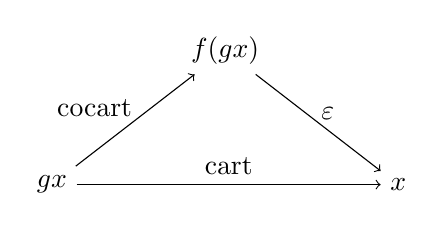
\begin{tikzpicture}
  \node (top) at (2.2,0) {$f(gx)$};
  \node (bl) at (0,-1.7) {$gx$};
  \node (br) at (4.4,-1.7) {$x$};
  \draw[->] (bl) -- node[above left, inner sep=1pt] {cocart} (top);
  \draw[->] (top) -- node[above right, inner sep=1pt] {$\varepsilon$} (br);
  \draw[->] (bl) -- node[above] {cart} (br);
\end{tikzpicture}
\end{center}
而我们刚刚验证过，任何一个复合都是笛卡尔边 $gx \to x$。
\end{proof}

\begin{remark}\label{rem:left-adjoint-criterion}
同样地，对 $\D$ 的每个\trObject{} $x$ 指定 $gx$ 以及映射 $x \to f(gx)$，使得
复合
\[
\mathrm{map}_{\C}(gx, z) \longrightarrow \mathrm{map}_{\D}(f(gx), f(z))
  \longrightarrow \mathrm{map}_{\D}(x, f(z))
\]
对一切 $z \in \C$ 都是一个\trEquivalence{}，便导致一个\trFunctor{} $g$，它是
$f$ 的\trLeftAdjoint{}，并且所指定的映射等价于该\trAdjunction{}的\trUnit{}。
\end{remark}

\begin{proposition}\label{prop:free-groupoid-left-adjoint}
对应 $\C \mapsto \C[W^{-1}]$——其中 $W$ 由 $\C$ 的全部\trMorphism{}组成——扩充为
包含 $\mathrm{Spc} \to \mathrm{Cat}_{\infty}$ 的一个\trLeftAdjoint{}。
\end{proposition}

\begin{proof}
由\cref{prop:right-adjoint-criterion}及其关于\trLeftAdjoint{}存在性的变体，只需
对每个
∞-\trCategory{} $\C$ 指定∞-\trGroupoid{} $\C[W^{-1}]$ 连同映射
$\C \to \C[W^{-1}]$，并证明：对每个∞-\trGroupoid{} $X$，复合
\[
\mathrm{map}_{\mathrm{Spc}}(\C[W^{-1}], X)
  \longrightarrow \mathrm{map}_{\mathrm{Cat}_{\infty}}(\C[W^{-1}], X)
  \longrightarrow \mathrm{map}_{\mathrm{Cat}_{\infty}}(\C, X)
\]
是一个\trEquivalence{}。如我们已经见过的，\trFunctor{}%
$\mathrm{Spc} \to \mathrm{Cat}_{\infty}$ 是\trFullyFaithful{}，故第一个映射是
一个\trEquivalence{}。接下来，我们回忆：对任意的∞-\trCategories{} $\C$ 与
$\D$，我们有
\[
\mathrm{map}_{\mathrm{Cat}_{\infty}}(\C, \D) \simeq
  \mathrm{Fun}(\C, \D)^{\simeq}.
\]
然而，如果 $\D$ 是一个∞-\trGroupoid{}，那么 $\mathrm{Fun}(\C, \D)$ 也是一个
∞-\trGroupoid{}，于是只需证明：映射
\[
\mathrm{Fun}(\C[W^{-1}], X) \simeq \mathrm{Fun}(\C, X)
\]
对一切∞-\trGroupoid{}都是一个\trEquivalence{}。\trLocalization{}的%
\trUniversalProperty{}表明，前者典范地等价于 $\mathrm{Fun}^{\simeq}(\C, X)$，即
$\mathrm{Fun}(\C, X)$ 中由把一切\trMorphism{}都送到\trEquivalence{}的那些%
\trFunctor{}组成的满子范畴。由于 $X$ 中的每个\trMorphism{}都是一个%
\trEquivalence{}，包含 $\mathrm{Fun}^{\simeq}(\C, X) \to \mathrm{Fun}(\C, X)$
是一个\trEquivalence{}。至此，本命题得证。
\end{proof}

下一个命题确保：如果我们已经有了一个\trRightAdjoint{}\trFunctor{}的候选者，那么
它就真的是一个\trRightAdjoint{}。

\begin{proposition}\label{prop:right-adjoint-counit-candidate}
设 $f\colon \C \to \D$ 与 $g\colon \D \to \C$ 是\trFunctor{}，并设
$\varepsilon\colon fg \to \mathrm{id}$ 是一个\trNaturalTransformation{}，使得
诱导的映射
\[
\mathrm{map}(x, g(y)) \longrightarrow \mathrm{map}(f(x), f(g(y)))
  \longrightarrow \mathrm{map}(f(x), y)
\]
对一切 $x$ 与 $y$ 都是一个\trEquivalence{}。那么，$g$ 是 $f$ 的\trRightAdjoint{}。
\end{proposition}

\begin{proof}
由\cref{prop:right-adjoint-criterion}，存在一个\trFunctor{} $g'$，它是 $f$ 的%
\trRightAdjoint{}，逐点等价于 $g$，并且其\trCounit{}映射等价于所选的映射。现在
我们还需
证明 $g'$ 等价于 $g$。为此，我们首先按下述办法构造一个\trNaturalTransformation{}%
$g \to g'$：我们回忆，通过与\trYoneda{}函子后合成而给出的\trFunctor{}%
$\mathrm{Fun}(\D, \C) \to \mathrm{Fun}(\D, \mathcal{P}(\C))$ 是%
\trFullyFaithful{}；于是，只需在 $g$ 与 $g'$ 的像之间构造一个\trEquivalence{}，
这两个像由如下两个\trFunctor{}给出：
\[
d \mapsto
\begin{cases}
\mathrm{map}_{\D}(f(-), d) & \text{对于 } g', \\
\mathrm{map}_{\C}(-, g(d)) & \text{对于 } g.
\end{cases}
\]
由\cref{ex:epsilon-natural-in-x}，我们发现这两个\trFunctor{}是等价的。于是，我们可以推出 $g$ 与 $g'$
也是等价的。
\end{proof}

\begin{corollary}\label{cor:right-adjoint-triangle-identities}
设 $f\colon \C \to \D$ 与 $g\colon \D \to \C$ 是\trFunctor{}。那么，$g$ 是 $f$
的\trRightAdjoint{}，当且仅当存在满足三角形恒等式（triangle identities）的%
\trUnit{}变换与\trCounit{}变换。
\end{corollary}

\begin{proof}
\trAdjunction{}满足三角形恒等式这一事实留给读者作为练习。反之，由前一个命题即得，
因为满足三角形恒等式蕴含：典范映射
\[
\mathrm{map}(x, g(y)) \longrightarrow \mathrm{map}(f(x), f(g(y)))
  \longrightarrow \mathrm{map}(f(x), y)
\]
是一个\trEquivalence{}，而它的一个逆由复合
\[
\mathrm{map}(f(x), y) \longrightarrow \mathrm{map}(gfx, gy)
  \longrightarrow \mathrm{map}(x, g(y)).
\]
给出。
\end{proof}

基于这一结果，我们可以证明下述关于\trAdjunction{}与\trDwyer{}--\trKan{}局部化
及函子范畴相容性的结果。

\begin{proposition}\label{prop:adjunction-localization}
设 $f\colon \C \to \D$ 与 $g\colon \D \to \C$。设 $\C$ 带有一个由\trMorphism{}%
组成的集合 $S$，而 $\D$ 带有一个由\trMorphism{}组成的集合 $T$。如果
$f(S) \subseteq T$ 且 $g(T) \subseteq S$，那么存在被诱导出的\trFunctor{}%
$F\colon \C[S^{-1}] \to \D[T^{-1}]$ 与 $G\colon \D[T^{-1}] \to \C[S^{-1}]$。
此外，如果 $f$ 是 $g$ 的\trLeftAdjoint{}，那么 $F$ 是 $G$ 的\trLeftAdjoint{}。
\end{proposition}

\begin{proof}
由\cref{cor:right-adjoint-triangle-identities}，只需构造满足三角形恒等式的变换
$FG \to \mathrm{id}$ 与 $\mathrm{id} \to GF$。我们先构造映射
$\mathrm{id} \to GF$，它是 $\mathrm{Fun}(\C[S^{-1}], \C[S^{-1}])$ 中从
$\mathrm{id}$ 到复合 $GF$ 的一条 $1$-\trSimplex{}。我们知道，限制\trFunctor{}%
\[
\ell^*\colon \mathrm{Fun}(\C[S^{-1}], \C[S^{-1}])
  \longrightarrow \mathrm{Fun}(\C, \C[S^{-1}])
\]
是\trFullyFaithful{}，故只需在后一个范畴中构造所要的那条 $1$-\trSimplex{}，即
从 $\ell$ 到 $GF \circ \ell$ 的那条。此外，还有一个\trFunctor{}%
\[
\mathrm{Fun}(\C, \C) \longrightarrow \mathrm{Fun}(\C, \C[S^{-1}])
\]
它由与\trLocalization{}映射 $\ell\colon \C \to \C[S^{-1}]$ 后合成而给出。该%
\trAdjunction{}的\trUnit{} $\eta$ 是前一个范畴中从 $\mathrm{id}$ 到 $gf$ 的一条
$1$-\trSimplex{}，于是这个\trFunctor{}给出 $\mathrm{Fun}(\C, \C[S^{-1}])$ 中从
$\ell$ 到 $\ell \circ gf$ 的一条 $1$-\trSimplex{}。由 $G$ 与 $F$ 的定义，存在
一个\trEquivalence{} $\ell \circ gf \simeq GF \circ \ell$。于是，我们便如所需地
找到了从 $\ell$ 到 $GF \circ \ell$ 的一个变换。同样地，可以得到\trCounit{}变换
$FG \to \mathrm{id}$。为了看出三角形恒等式成立，我们考虑在下述图表中见证 $f$ 的
三角形恒等式的那个 $2$-\trSimplex{}%
\[
\begin{aligned}
\Delta^2 &\longrightarrow \mathrm{map}_{\mathrm{Fun}(\C, \D)}(f, f) \\
&\longrightarrow
  \mathrm{map}_{\mathrm{Fun}(\C, \D[T^{-1}])}(\ell_\D \circ f,\ \ell_\D \circ f) \\
&\xleftarrow{\ \simeq\ }
  \mathrm{map}_{\mathrm{Fun}(\C[S^{-1}], \D[T^{-1}])}(F, F)
\end{aligned}
\]
注意，所得的 $\mathrm{map}(F, F)$ 的那个 $2$-\trSimplex{}见证了 $F$ 的三角形
恒等式。关于 $G$ 的论证是类似的。
\end{proof}

\begin{proposition}\label{prop:adjoint-functor-categories}
设 $f\colon \C \to \D$ 是一个\trFunctor{}，$K$ 是一个\trSimplicialSet{}，$\E$ 是
一个辅助的∞-\trCategory{}。如果 $f$ 容许一个\trRightAdjoint{}或%
\trLeftAdjoint{}，那么 $f_*\colon \mathrm{Fun}(K, \C) \to \mathrm{Fun}(K, \D)$
亦然。如果 $f$ 容许一个\trRightAdjoint{}或\trLeftAdjoint{}，那么
$f^*\colon \mathrm{Fun}(\D, \E) \to \mathrm{Fun}(\C, \E)$ 分别容许一个%
\trLeftAdjoint{}或\trRightAdjoint{}。
\end{proposition}

\begin{proof}
设 $g$ 是 $f$ 的一个\trRightAdjoint{}。我们证明 $g_*$ 是 $f_*$ 的%
\trRightAdjoint{}，而
$g^*$ 是 $f^*$ 的\trLeftAdjoint{}；其余情形是类似的。为此，设
$\varepsilon\colon fg \to \mathrm{id}$
是该\trAdjunction{}的\trCounit{}，$\eta\colon \mathrm{id} \to gf$
是其\trUnit{}，把它们视为\trMorphism{}%
\[
\Delta^1 \xrightarrow{\ \varepsilon\ } \mathrm{Fun}(\D, \D)
\qquad\qquad
\Delta^1 \xrightarrow{\ \eta\ } \mathrm{Fun}(\C, \C).
\]
于是，我们可以与典范\trFunctor{}%
$\mathrm{Fun}(\C, \D) \to \mathrm{Fun}(\C^K, \D^K)$ 后合成，得到新的变换
$\varepsilon_*\colon f_*g_* \to \mathrm{id}_*$ 与
$\eta_*\colon \mathrm{id}_* \to g_*f_*$。容易验证，这些变换满足三角形恒等式，
从而构成一个\trAdjunction{}。同样地，可以与\trFunctor{}%
$\mathrm{Fun}(\C, \D) \to \mathrm{Fun}(\E^{\D}, \E^{\C})$ 合成，得到变换
$\varepsilon^*\colon (fg)^* = g^*f^* \to \mathrm{id}^*$ 与
$\eta^*\colon \mathrm{id}^* \to (gf)^* = f^*g^*$。这些变换同样满足三角形
恒等式，于是 $g^*$ 是 $f^*$ 的\trLeftAdjoint{}。
\end{proof}

\begin{corollary}\label{cor:maximal-groupoid-right-adjoint}
由取极大子∞-群胚而给出的\trFunctor{}%
$\mathrm{Cat}_{\infty} \to \mathrm{Spc}$ 是包含
$\mathrm{Spc} \to \mathrm{Cat}_{\infty}$ 的一个\trRightAdjoint{}。
\end{corollary}

\begin{proof}
包含\trFunctor{} $\mathrm{Kan} \to \mathrm{Cat}^1_{\infty}$ 有一个%
\trRightAdjoint{}，由 $\mathrm{Cat}^1_{\infty} \to \mathrm{Kan}$ 给出，它把 $\C$
送到 $\C^{\simeq}$。该包含把\trHomotopyEquivalence{}送到\trJoyalEquivalence{}，
而极大子群胚\trFunctor{}把\trJoyalEquivalence{}送到\trHomotopyEquivalence{}。
于是，我们可以应用\cref{prop:adjunction-localization}。
\end{proof}

\begin{remark}\label{rem:maximal-groupoid-via-counit}
当然，我们也可以利用\cref{prop:right-adjoint-counit-candidate}来证明%
\cref{cor:maximal-groupoid-right-adjoint}。此时，对∞-\trGroupoid{} $X$ 与
∞-\trCategory{} $\C$，必须证明典范映射
\[
\mathrm{Fun}(X, \C^{\simeq}) \longrightarrow \mathrm{Fun}(X, \C)^{\simeq}
\]
是一个\trHomotopyEquivalence{}。
\end{remark}

\begin{proposition}\label{prop:bousfield-right-adjoint-ff}
设 $\ell\colon \C \to \D$ 是一个\trDwyer{}--\trKan{}\trLocalization{}。假设
$\ell$ 容许一个\trRightAdjoint{} $r$。那么 $r$ 是\trFullyFaithful{}。
\end{proposition}

\begin{proof}
我们断言，在∞-\trCategory{} $\mathrm{Cat}_{\infty}$ 中存在一个交换图表
\begin{center}
\begin{tikzpicture}
  \node (d) at (0,0) {$\D$};
  \node (c) at (3.6,0) {$\C$};
  \node (pd) at (0,-2.0) {$\mathcal{P}(\D)$};
  \node (pc) at (3.6,-2.0) {$\mathcal{P}(\C)$};
  \draw[->] (d) -- node[above] {$r$} (c);
  \draw[->] (d) -- node[right] {$y_\D$} (pd);
  \draw[->] (c) -- node[right] {$y_\C$} (pc);
  \draw[->] (pd) -- node[above] {$\ell^*$} (pc);
\end{tikzpicture}
\end{center}
对它我们必须核验：在\trFunctor{}%
\[
d \mapsto
\begin{cases}
c \mapsto \mathrm{map}_{\C}(c, r(d)), \\
c \mapsto \mathrm{map}_{\D}(\ell(c), d)
\end{cases}
\]
之间是否存在一个\trNaturalEquivalence{}。而这正是「$r$ 是 $\ell$ 的%
\trRightAdjoint{}」这一
事实的推论，见\cref{prop:adjunction-map-natural-equivalence}。由于 $\ell$ 是一个%
\trLocalization{}，\trFunctor{} $\ell^*$ 是\trFullyFaithful{}。于是，本命题由
「\trYoneda{}函子是\trFullyFaithful{}」这一事实即得。
\end{proof}

\begin{definition}\label{def:bousfield-localization}
容许一个\trRightAdjoint{}的\trDwyer{}--\trKan{}\trLocalization{}称为一个%
\emph{\trBousfield{}\trLocalization{}}（Bousfield localization）。
\end{definition}

\begin{definition}\label{def:essentially-locally-small}
一个∞-\trCategory{}称为\emph{\trEssentiallySmall{}}（essentially small），如果
它等价于一个小的∞-\trCategory{}。一个∞-\trCategory{}称为%
\emph{\trLocallySmall{}}（locally small），如果对 $\C$ 的任何两个\trObject{}%
$x$ 与 $y$，\trMappingSpace{} $\mathrm{map}_{\C}(x, y)$ 是%
\trEssentiallySmall{}。
\end{definition}

\begin{corollary}\label{cor:bousfield-locally-small}
设 $\C$ 是一个\trLocallySmall{}∞-\trCategory{}，并设 $\C \to \D$ 是一个%
\trBousfield{}\trLocalization{}。那么 $\D$ 是\trLocallySmall{}。
\end{corollary}

\begin{proof}
由\cref{prop:bousfield-right-adjoint-ff}，$\D$ 可以等同于 $\C$ 的一个满子范畴，
因此它也是\trLocallySmall{}。
\end{proof}

\begin{proposition}\label{prop:ff-right-adjoint-bousfield}
设 $f\colon \C \to \D$ 是任何一个容有\trFullyFaithful{}\trRightAdjoint{} $r$
的%
\trFunctor{}。那么 $f$ 是一个\trBousfield{}\trLocalization{}。
\end{proposition}

\begin{proof}
由\cref{prop:bousfield-right-adjoint-ff}，只需证明 $f$ 是一个\trDwyer{}--%
\trKan{}\trLocalization{}。设 $\E$ 是一个辅助的∞-\trCategory{}。我们需要证明：
\trFunctor{} $f^*\colon \mathrm{Fun}(\D, \E) \to \mathrm{Fun}(\C, \E)$ 是%
\trFullyFaithful{}，并刻画其\trEssentialImage{}。为了看出 $f^*$ 是%
\trFullyFaithful{}，我们观察到：由\cref{prop:adjoint-functor-categories}，
$r^*$ 是 $f^*$ 的一个\trLeftAdjoint{}。此外，由假设，$fr \to \mathrm{id}$ 是
一个\trEquivalence{}。由构造，我们发现 $r^*f^* \to \mathrm{id}$ 也是一个%
\trEquivalence{}，从而 $f^*$ 是\trFullyFaithful{}。剩下还需证明 $f$ 是一个%
\trDwyer{}--\trKan{}\trLocalization{}。如果是这样，那么它必定是沿 $f$-等价之集
的\trDwyer{}--\trKan{}\trLocalization{}，也就是说，沿那些在施加 $f$ 之后变为
等价的\trMorphism{}。于是，我们需要考虑一个具有如下性质的\trFunctor{}%
$a\colon \C \to \E$：它把 $f$-等价送到等价；并证明它等价于某个\trFunctor{}%
$b\colon \D \to \E$ 的复合 $\C \to \D \to \E$。我们断言 $b = ar$ 可行。为了
确证这一断言，我们必须证明 $a$ 与 $arf$ 之间存在一个\trEquivalence{}。该%
\trAdjunction{}的\trUnit{}是一个映射 $\mathrm{id} \to rf$，我们断言它由
$f$-等价组成：把 $f$ 应用到映射 $x \to rf(x)$ 上，得到一个映射
$fx \to frf(x)$，我们可以将它与\trCounit{}后合成，得到复合
$fx \to frf(x) \to f(x)$。由三角形恒等式，该复合是一个\trEquivalence{}，而%
\trRightAdjoint{} $r$ 是\trFullyFaithful{}这一事实蕴含\trCounit{}是一个%
\trEquivalence{}，见\cref{prop:cart-cocart-fully-faithful}。于是，\trUnit{}是
一条 $f$-等价。于是，
「$a$ 把 $f$-等价送到等价」这一事实便蕴含：典范映射 $a \to arf$ 如所需要地是
一个\trEquivalence{}。
\end{proof}

\begin{example*}
由逆转全部\trMorphism{}而给出的\trFunctor{}%
$\mathrm{Cat}_{\infty} \to \mathrm{Spc}$ 有一个\trFullyFaithful{}%
\trRightAdjoint{}，由包含
$\mathrm{Spc} \to \mathrm{Cat}_{\infty}$ 给出。于是，它是一个%
\trBousfield{}\trLocalization{}。
\end{example*}

\begin{proposition}\label{prop:colimit-adjoint}
设 $\C$ 是一个∞-\trCategory{}，$K$ 是一个\trSimplicialSet{}。如果 $\C$ 容许
$K$-指标化的\trColimit{}，那么它们的构造装配成一个\trFunctor{}%
$\mathrm{colim}_K\colon \mathrm{Fun}(K, \C) \to \C$，它是常值\trFunctor{}的左
伴随。反之，如果常值\trFunctor{}%
$\mathrm{const}\colon \C \to \mathrm{Fun}(K, \C)$ 容许一个\trLeftAdjoint{}%
$F$，那么对任何图表 $p\colon K \to \C$，$F(p)$ 都是 $p$ 的一个\trColimit{}。
\end{proposition}

\begin{proof}
对于\trLeftAdjoint{}存在性的证明，我们采用\cref{rem:left-adjoint-criterion}。
于是，我们
首先必须对 $\mathrm{Fun}(K, \C)$ 的每个\trObject{} $p$，指定 $\C$ 的一个%
\trObject{} $t$ 以及一个映射 $p \to \mathrm{const}(t)$。作为\trObject{}，我们
选取一个\trColimit{} $\mathrm{colim}_K\, p$。于是，我们需要在
$\mathrm{Fun}(K, \C)$ 中构造一个\trMorphism{}%
$p \to \mathrm{const}(\mathrm{colim}_K\, p)$，其中
$\mathrm{const}(\mathrm{colim}_K\, p)$ 是取值 $\mathrm{colim}_K\, p$ 的常值%
\trFunctor{}。由伴随性，这样一个\trMorphism{}是一个映射
$K \times \Delta^1 \to \C$。选取一个\trColimit{}\trCone{}%
$\bar{p}\colon K \diamond \Delta^0 \to \C$，我们可以沿典范映射
$K \times \Delta^1 \to K \diamond \Delta^0$ 限制它。由构造，限制到
$K \times \{0\}$ 上给出 $p$，而限制到 $K \times \{1\}$ 上则如所需要地给出取值
$\bar{p}(\infty)$ 的常值\trFunctor{}。于是，我们必须证明：复合映射
\[
\begin{aligned}
\mathrm{map}_{\C}(\mathrm{colim}_K\, p, x)
  &\to \mathrm{map}_{\mathrm{Fun}(K, \C)}\\
&\quad (\mathrm{const}(\mathrm{colim}_K\, p), \mathrm{const}(x))
  \to \mathrm{map}_{\mathrm{Fun}(K, \C)}(p, \mathrm{const}(x))
\end{aligned}
\]
是一个\trEquivalence{}。在\cref{prop:map-fun-mapping-space}的诸\trEquivalence{}%
之下，该映射对应于典范映射
\[
\mathrm{map}_{\C}(\mathrm{colim}_K\, p, x)
  \xleftarrow{\ \simeq\ } \mathrm{Map}(\bar{p}, x)
  \longrightarrow \mathrm{Map}(p, x),
\]
而由「$\bar{p}$ 是一个\trColimit{}\trCone{}」这一假设，它是一个%
\trEquivalence{}。

反之，假设常值\trFunctor{}容许一个\trLeftAdjoint{}%
$F\colon \mathrm{Fun}(K, \C) \to \C$，并考虑一个\trFunctor{} $p\colon K \to \C$。
我们想证明 $F(p)$ 是 $p$ 的一个\trColimit{}。为此，首先注意：该\trAdjunction{}%
的\trUnit{}给出 $\mathrm{Fun}(K, \C)$ 中的一个映射
$p \to \mathrm{const}\, F(p)$。这个映射伴随于一个映射
$K \times \Delta^1 \to \C$，并且与前面一样，容易验证该映射穿过投射
$K \times \Delta^1 \to K \diamond \Delta^0$ 而分解。所得的映射
$\bar{p}\colon K \diamond \Delta^0 \to \C$ 是 $p$ 之上的一个\trCone{}，剩下还需
证明它是一个\trInitialCone{}（initial cone）。而这成立，当且仅当典范映射
\[
\mathrm{Map}_{\C}(\bar{p}, x) \to \mathrm{Map}_{\C}(p, x) \simeq
\mathrm{map}_{\C^K}(p, \mathrm{const}_x) \simeq
\mathrm{map}_{\C}(F(p), x)
\]
是一个\trEquivalence{}。但在这里同样地，该复合等价于沿包含
$\{\infty\} \to K \diamond \Delta^0$ 限制而给出的那个典范映射，而后者是一个%
\trEquivalence{}。
\end{proof}

\begin{remark}\label{rem:limit-adjoint-dual}
对偶地，同样的陈述对\trLimit{}成立：如果可能的话，\trLimit{}的构造是一个%
\trFunctor{}，它是常值\trFunctor{}的\trRightAdjoint{}。
\end{remark}

\begin{definition}\label{def:K-cocomplete}
设 $\mathcal{K}$ 是一个由\trSimplicialSets{}组成的集合。我们说一个∞-\trCategory{}%
是 $\mathcal{K}$-（余）完备的，如果它容许一切 $K$-指标化的（余）\trLimit{}，
也就是说，对含于 $\mathcal{K}$ 中的\trSimplicialSets{} $K$ 指标化的那些
（余）\trLimit{}。
\end{definition}

\begin{proposition}\label{prop:fun-K-cocomplete}
设 $\C$ 是一个 $\mathcal{K}$-余完备的（相应地，$\mathcal{K}$-完备的）
∞-\trCategory{}，$L$ 是一个\trSimplicialSet{}。那么 $\mathrm{Fun}(L, \C)$ 仍是
$\mathcal{K}$-余完备的（相应地，$\mathcal{K}$-完备的）。
\end{proposition}

\begin{proof}
设 $K$ 是 $\mathcal{K}$ 的一个元素。我们断言：复合
\[
\mathrm{Fun}(K, \mathrm{Fun}(L, \C)) \simeq
  \mathrm{Fun}(L, \mathrm{Fun}(K, \C)) \longrightarrow \mathrm{Fun}(L, \C),
\]
其中后一个\trFunctor{}是与\trColimit{}\trFunctor{}%
$\mathrm{colim}_K\colon \mathrm{Fun}(K, \C) \to \C$ 的后合成，是常值\trFunctor{}%
的\trLeftAdjoint{}。由「$(\mathrm{colim}_K)_*$ 是 $\mathrm{const}_*$ 的%
\trLeftAdjoint{}」这一事实
（\cref{prop:adjoint-functor-categories}），这一点立即得出。\footnote{译注：原书%
此处作「右伴随」，与其前句「左伴随」及命题 5.1.16 的伴随方向不合，径改。
——译者注}
\end{proof}

\begin{corollary}\label{cor:const-preserves-K-colimits}
设 $\C$ 是 $\mathcal{K}$-（余）完备的，并设 $L$ 是一个\trSimplicialSet{}。那么，
常值\trFunctor{} $\C \to \mathrm{Fun}(L, \C)$ 保持 $\mathcal{K}$-指标化的
（余）\trLimit{}。
\end{corollary}

\begin{proof}
我们想证明：如果 $K$ 含于 $\mathcal{K}$，而 $p\colon K \to \C$ 是一个带有%
\trColimit{} $x$ 的图表，那么取值 $x$ 的常值\trFunctor{}是图表
$K \to \C \to \mathrm{Fun}(L, \C)$ 的一个\trColimit{}。为此，我们首先观察到：
对任何\trFunctor{} $\varphi\colon \D \to \E$ 与任何\trSimplicialSet{} $S$，
图表
\begin{center}
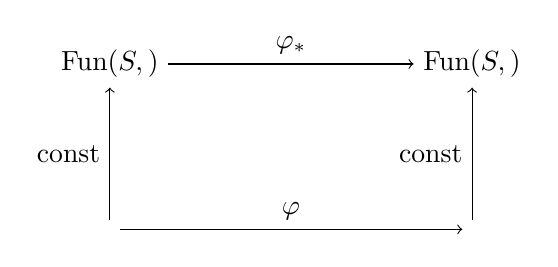
\begin{tikzpicture}
  \node (tl) at (0,0) {$\mathrm{Fun}(S, \D)$};
  \node (tr) at (4.6,0) {$\mathrm{Fun}(S, \E)$};
  \node (bl) at (0,-2.1) {$\D$};
  \node (br) at (4.6,-2.1) {$\E$};
  \draw[->] (tl) -- node[above] {$\varphi_*$} (tr);
  \draw[->] (bl) -- node[left] {const} (tl);
  \draw[->] (br) -- node[left] {const} (tr);
  \draw[->] (bl) -- node[above] {$\varphi$} (br);
\end{tikzpicture}
\end{center}
交换。把这个观察应用到\trFunctor{}%
$\mathrm{colim}_K\colon \mathrm{Fun}(K, \C) \to \C$ 与\trSimplicialSet{} $L$
之上，我们便得到交换图表
\begin{center}
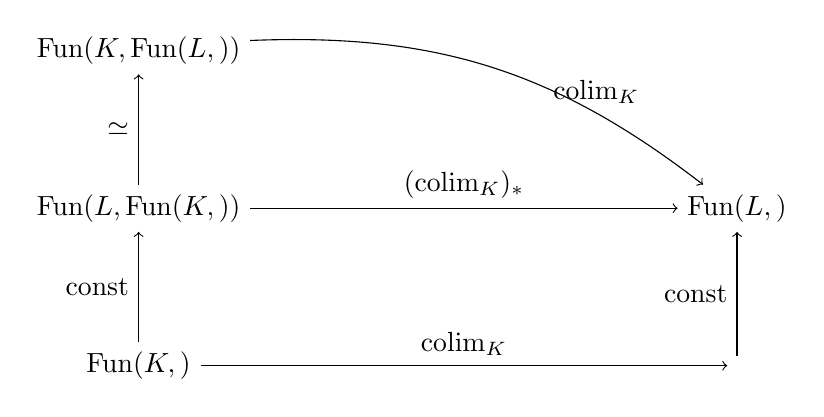
\begin{tikzpicture}
  \node (a) at (0,2.0) {$\mathrm{Fun}(K, \mathrm{Fun}(L, \C))$};
  \node (c) at (0,0) {$\mathrm{Fun}(L, \mathrm{Fun}(K, \C))$};
  \node (e) at (0,-2.0) {$\mathrm{Fun}(K, \C)$};
  \node (b) at (7.6,0) {$\mathrm{Fun}(L, \C)$};
  \node (f) at (7.6,-2.0) {$\C$};
  \draw[->, bend left=20] (a) to node[above, pos=0.75]
    {$\mathrm{colim}_K$} (b);
  \draw[->] (c) -- node[above] {$(\mathrm{colim}_K)_*$} (b);
  \draw[->] (c) -- node[left] {$\simeq$} (a);
  \draw[->] (e) -- node[left] {const} (c);
  \draw[->] (e) -- node[above] {$\mathrm{colim}_K$} (f);
  \draw[->] (f) -- node[left] {const} (b);
\end{tikzpicture}
\end{center}
其中左边的竖直复合由与常值\trFunctor{} $\C \to \mathrm{Fun}(L, \C)$ 的后合成
给出。注意，上方的三角形由\cref{prop:fun-K-cocomplete}的证明可交换。于是，该
图表的交换性便蕴含本推论的陈述。
\end{proof}

\begin{proposition}\label{prop:left-adjoint-preserves-colimits}
设 $f\colon \C \to \D$ 是一个\trLeftAdjoint{}。那么 $f$ 保持\trColimit{}。同样地，
\trRightAdjoint{}保持\trLimit{}。
\end{proposition}

\begin{proof}
我们只证明\trLeftAdjoint{}保持\trColimit{}；另一种情形可以通过取%
\trOppositeCategory{}得到。
于是，设
$F\colon K \to \C$ 是一个图表，$\bar{F}$ 是一个\trColimit{}\trCone{}。我们想
证明 $f\bar{F}$ 是 $fF$ 的一个\trColimit{}\trCone{}，而这等于要对 $\D$ 的一个%
\trObject{} $z$ 证明：典范映射
\[
\mathrm{Map}_{\D}(f\bar{F}, z) \longrightarrow \mathrm{Map}_{\D}(fF, z)
\]
是一个\trEquivalence{}。为此，我们断言：对任何\trFunctor{} $G\colon L \to \C$，
存在一个典范的\trEquivalence{}%
\[
\mathrm{Map}_{\D}(fG, z) \simeq \mathrm{Map}_{\C}(G, gz),
\]
其中 $g$ 是 $f$ 的\trRightAdjoint{}。暂时把这个断言当作给定的，我们随后考虑
交换图表
\begin{center}
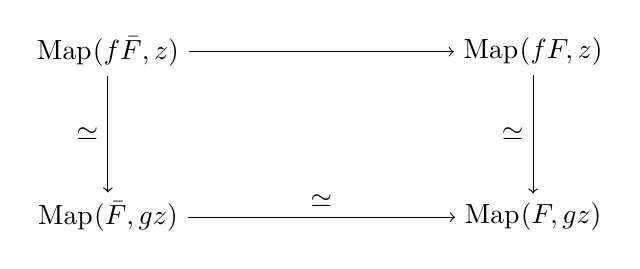
\begin{tikzpicture}
  \node (tl) at (0,0) {$\mathrm{Map}_{\D}(f\bar{F}, z)$};
  \node (tr) at (5.4,0) {$\mathrm{Map}_{\D}(fF, z)$};
  \node (bl) at (0,-2.1) {$\mathrm{Map}_{\C}(\bar{F}, gz)$};
  \node (br) at (5.4,-2.1) {$\mathrm{Map}_{\C}(F, gz)$};
  \draw[->] (tl) -- (tr);
  \draw[->] (tl) -- node[left] {$\simeq$} (bl);
  \draw[->] (tr) -- node[left] {$\simeq$} (br);
  \draw[->] (bl) -- node[above] {$\simeq$} (br);
\end{tikzpicture}
\end{center}
其中诸竖直映射由该断言是\trEquivalence{}，而下方的水平映射由「$\bar{F}$ 是一个%
\trColimit{}\trCone{}」这一假设是\trEquivalence{}。于是，上方的映射如所需要地
也是一个\trEquivalence{}。

剩下还需证明该断言。为此，我们考虑下述等价链：
\[
\begin{aligned}
\mathrm{Map}_{\D}(fG, z)
  &\simeq \mathrm{map}_{\D^K}(f_*(G), \mathrm{const}_z)
  && \text{由\cref{prop:map-fun-mapping-space}} \\
&\simeq \mathrm{map}_{\C^K}(G, g_*(\mathrm{const}_z))
  && \text{由\cref{prop:adjoint-functor-categories}} \\
&\simeq \mathrm{map}_{\C^K}(G, \mathrm{const}_{gz})
  && \text{因为 } g_*(\mathrm{const}_z) = \mathrm{const}_{gz} \\
&\simeq \mathrm{Map}_{\C}(G, gz)
  && \text{由\cref{prop:map-fun-mapping-space}}
\end{aligned}
\]
\end{proof}

最后，为了在下一节中建立\trAdjointFunctorTheorem{}，我们需要下述命题。

\begin{proposition}\label{prop:pullback-colimits}
考虑∞-\trCategories{}的一个\trPullback{}图表
\begin{center}
\begin{tikzpicture}
  \node (c) at (0,0) {$\C$};
  \node (cp) at (3.0,0) {$\C'$};
  \node (d) at (0,-2.0) {$\D$};
  \node (dp) at (3.0,-2.0) {$\D'$};
  \draw[->] (c) -- node[above] {$f$} (cp);
  \draw[->] (c) -- node[left] {$q$} (d);
  \draw[->] (cp) -- node[right] {$p$} (dp);
  \draw[->] (d) -- node[above] {$g$} (dp);
\end{tikzpicture}
\end{center}
其中映射 $p$ 是一个\trIsofibration{}。假设 $p$ 保持\trColimit{}，并设
$F\colon K \to \C$ 是一个图表。那么：
\begin{enumerate}[label=(\arabic*)]
  \item 一个\trCone{} $\bar{F}\colon K \diamond \Delta^0 \to \C$ 是一个%
        \trColimit{}\trCone{}，如果它在 $f$ 与 $q$ 之下的像是\trColimit{}%
        \trCone{}。
  \item 如果 $\C'$ 与 $\D$ 是\trCocomplete{}，而 $g$ 保持\trColimit{}，那么
        $\C$ 也是\trCocomplete{}。此外，$f$ 与 $q$ 保持\trColimit{}。
\end{enumerate}
\end{proposition}

\begin{proof}
首先要观察到的是：对 $\C$ 的任何\trObject{} $x$，存在一个%
\trHomotopyCartesian{}图表
\begin{center}
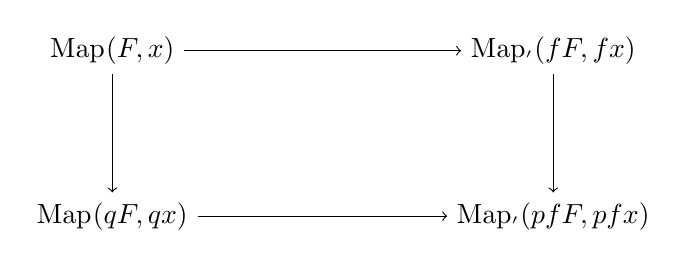
\begin{tikzpicture}
  \node (tl) at (0,0) {$\mathrm{Map}_{\C}(F, x)$};
  \node (tr) at (5.6,0) {$\mathrm{Map}_{\C'}(fF, fx)$};
  \node (bl) at (0,-2.1) {$\mathrm{Map}_{\D}(qF, qx)$};
  \node (br) at (5.6,-2.1) {$\mathrm{Map}_{\D'}(pfF, pfx)$};
  \draw[->] (tl) -- (tr);
  \draw[->] (tl) -- (bl);
  \draw[->] (tr) -- (br);
  \draw[->] (bl) -- (br);
\end{tikzpicture}
\end{center}
这由\cref{prop:map-fun-mapping-space}以及「\trPullback{}中的诸%
\trMappingSpace{}由诸\trMappingSpace{}的\trPullback{}给出」这一事实得出。
（注意，我们用到了这样一个事实：把\trFunctor{} $\mathrm{Fun}(K, -)$ 应用到上述
图表上仍给出一个\trPullback{}图表，并且其中一条腿是\trIsofibration{}。）

接下来，我们想分析 $\bar{F}$ 是否是一个\trColimit{}\trCone{}。为此，我们对
$\bar{F}$ 与 $F$ 考虑上面的那些正方形，便得到一个典范的交换立方体。「$f\bar{F}$
与 $q\bar{F}$ 是\trColimit{}\trCone{}」这一假设蕴含：左下角与右上角处的比较映射
是\trEquivalence{}。利用 $p$ 保持\trColimit{}这一事实，我们发现 $pf\bar{F}$ 也是
一个\trColimit{}\trCone{}，于是比较映射也是\trEquivalence{}。因此，比较映射在
左上角也是\trEquivalence{}，从而 $\bar{F}$ 是一个\trColimit{}\trCone{}。这就证明
了（1）。

为了证明（2），只需证明：任何图表 $F\colon K \to \C$ 都容有一个\trCone{}%
$\bar{F}$，使得它在 $\D$ 与 $\C'$ 中的像是\trColimit{}\trCone{}：一旦证明了
这一点，我们就可以应用（1）得出 $\bar{F}$ 是一个\trColimit{}\trCone{}，并且由
构造，$q$ 与 $f$ 又把 $\bar{F}$ 送到\trColimit{}\trCone{}。

为了证明上述陈述，我们考虑复合 $F_1\colon K \to \C \to \C'$ 并选取一个%
\trColimit{}\trCone{} $\bar{F}_1\colon K \diamond \Delta^0 \to \C'$。同样地，
我们考虑复合 $F_2\colon K \to \C \to \D$ 并选取一个\trColimit{}\trCone{}%
$\bar{F}_2\colon K \diamond \Delta^0 \to \D$。于是，由「$p$ 与 $g$ 都保持%
\trColimit{}」这一假设，像 $g\bar{F}_2$ 与 $p\bar{F}_1$ 也是\trColimit{}%
\trCone{}。因此，在这两个\trCone{}之间存在一个\trEquivalence{} $\tau$。我们
约定 $\tau$ 是从 $p\bar{F}_1$ 到 $g\bar{F}_2$ 的一个\trEquivalence{}。于是，
我们得到一个\trLiftingProblem{}%
\begin{center}
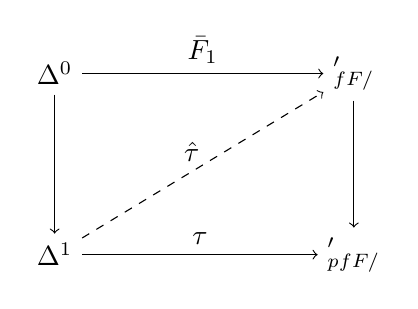
\begin{tikzpicture}
  \node (tl) at (0,0) {$\Delta^0$};
  \node (tr) at (3.8,0) {$\C'_{fF/}$};
  \node (bl) at (0,-2.3) {$\Delta^1$};
  \node (br) at (3.8,-2.3) {$\D'_{pfF/}$};
  \draw[->] (tl) -- node[above] {$\bar{F}_1$} (tr);
  \draw[->] (tl) -- (bl);
  \draw[->] (bl) -- node[above] {$\tau$} (br);
  \draw[->] (tr) -- (br);
  \draw[->, dashed] (bl) -- node[above left, inner sep=1pt]
    {$\hat{\tau}$} (tr);
\end{tikzpicture}
\end{center}
它容有一个解，因为右边的竖直映射是一个\trIsofibration{}（因为 $p$ 是一个%
\trIsofibration{}）。此外，这条虚箭头在 $\C'$ 中仍是一个\trEquivalence{}，从而
$\hat{\tau}(1)$ 是 $fF$ 的又一个\trCocone{}。把这些定义铺开来，我们便得到一个
交换图表
\begin{center}
\begin{tikzpicture}
  \node (tl) at (0,0) {$K \diamond \Delta^0$};
  \node (tr) at (3.8,0) {$\C'$};
  \node (bl) at (0,-2.0) {$\D$};
  \node (br) at (3.8,-2.0) {$\D'$};
  \draw[->] (tl) -- node[above] {$\hat{\tau}(1)$} (tr);
  \draw[->] (tl) -- node[left] {$\bar{F}_2$} (bl);
  \draw[->] (tr) -- node[right] {$p$} (br);
  \draw[->] (bl) -- node[above] {$g$} (br);
\end{tikzpicture}
\end{center}
这就给出一个唯一的映射 $K \diamond \Delta^0 \to \C$，如所断言的那样，它是
$F$ 之上的一个\trCone{}。
\end{proof}
